\cleardoublepage
\newpage
\ifdefined\EnableIncludeImages
    \ThisULCornerWallPaper{1.0}{chapterimage.eps}
\fi
\chapter{Zandor}

Após a morte de Zorra, toda a família ficou muito triste, pois apesar de seus maus costumes, ela sempre foi muito amorosa conosco; por isso, sentíamos sua falta como se fosse um membro da família. 
Assim, passamos muito tempo chorando, sobretudo minhas irmãs e eu, que ainda éramos crianças. 
Muitas vezes vi a Teodosia ---  minha irmã mais velha, a qual carinhosamente chamávamos ``Tulaco'' ---, iniciar a chorar em silêncio ao ver o lugar onde Zorra dormia; inclusive Diofelia  --- ``Dio'', a minha irmã mais nova ---, apesar de sua curta idade, já sabia distinguir a morte e a ausência que ela deixa. 
Eu também chorava, talvez mais do que elas, porque Zorra era minha companheira fiel, ela me seguia em todos os lugares onde eu ia; pois, ao ser o filho homem da casa, eu era quem tinha que sair para trabalhar na chacra com meu pai, e Zorra sempre fazia mais alegres e memoráveis esses momentos.
Nosso único conforto era que tínhamos o Zandor; nós o amávamos por ser o último presente que Zorra nos deixou.
Eu olhava para Zandor --- todo pequeno e pretinho --- e ficava maravilhado com o quanto era fofo. Sua presença me dizia que, de alguma forma, uma parte de Zorra ainda estava conosco. 
Assim, Zandor cresceu sendo criado com muito cuidado e carinho por todos nós;
entretanto, a personalidade de Zandor era completamente distinta da de sua mãe; ele era um cachorro muito honesto e era evidente para nós que ele não tinha nenhuma dos maus costumes de Zorra. 
\ifdefined\EnableIncludeImages
\begin{wrapfigure}{r}{0.45\textwidth}
  \begin{center}
  \vspace{-20pt}
    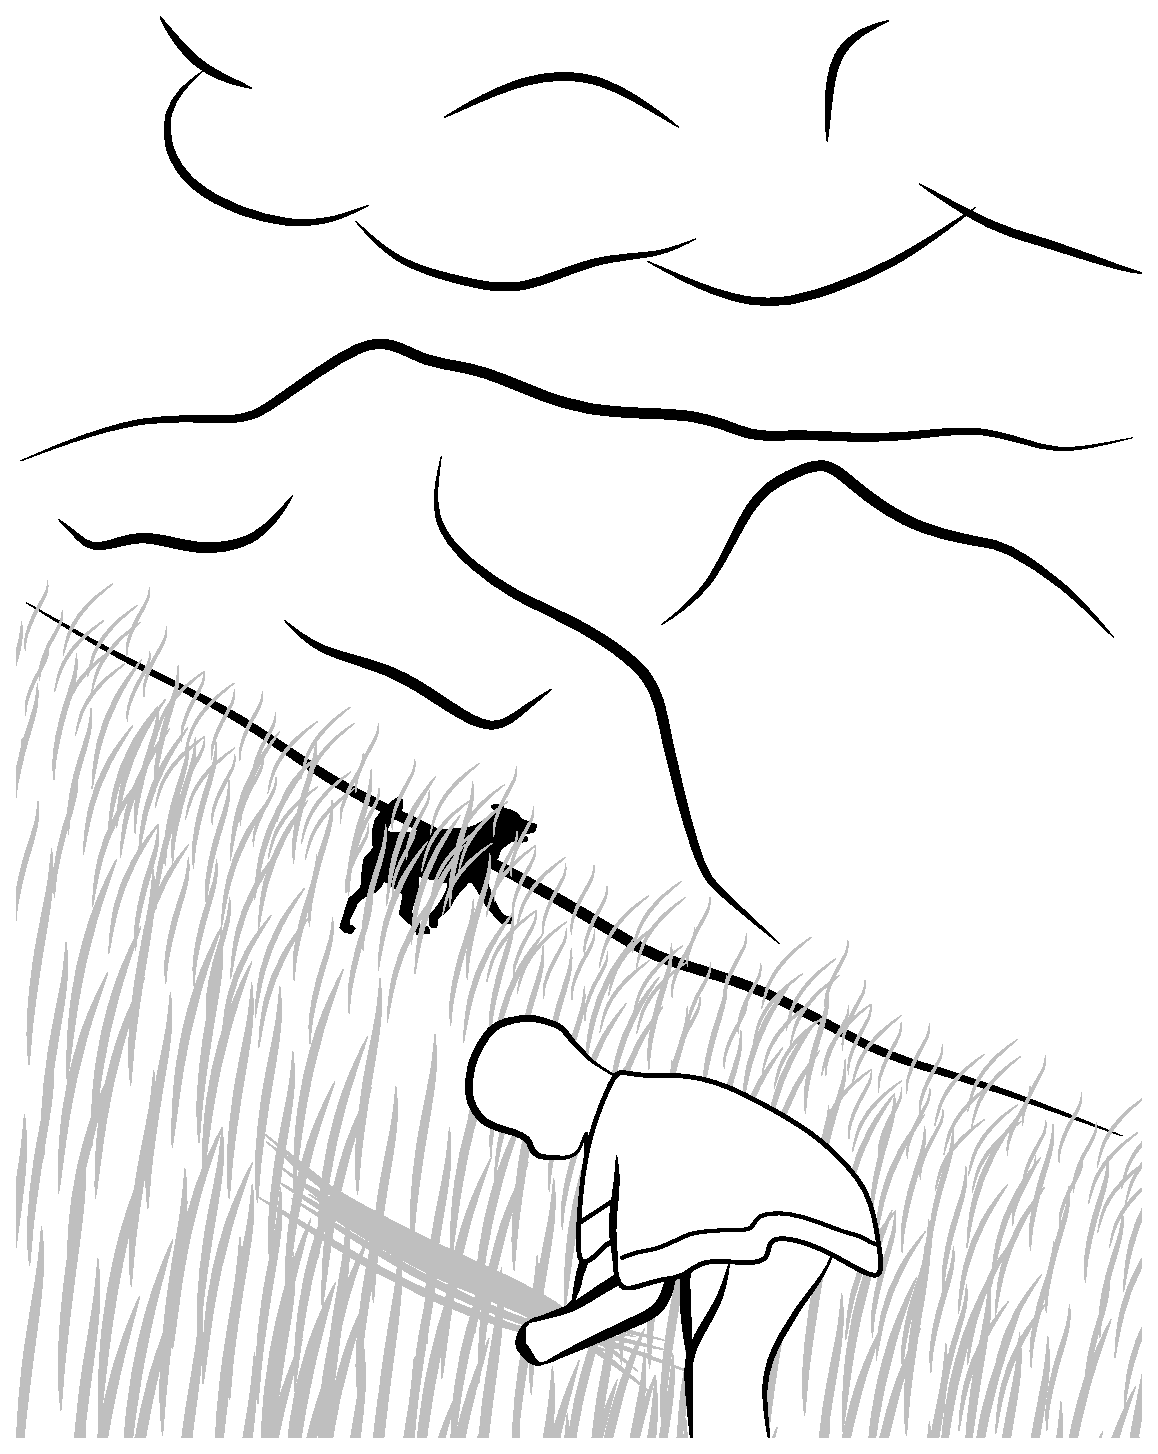
\includegraphics[width=0.43\textwidth]{pasto-zandor-aulicha}
  \end{center}
  \vspace{-20pt}
  %\caption{Figo das índias.}
\end{wrapfigure}
\fi
Desde pequeno eu levava Zandor a todas as minhas caminhadas pelo campo; como minha família tinha vacas, eu tinha que ir dar-lhes comida e atendê-las, e comumente recompensava Zandor por sua companhia dando-lhe leite fresco, que eu mesmo ordenhava para matar a nossa fome. 
Com todos esses cuidados, em pouco tempo Zandor virou um cachorrinho forte e muito brincalhão.
Ele me ajudava a cuidar das vacas e assustava os pássaros que vinham comer as sementes na chacra. Quando eu gritava seu nome, ele vinha correndo e se parava de frente a mim com a severidade de um soldado diante do seu general; ele era tão inteligente quanto uma pessoa e bem mais obediente que eu mesmo.

Um dia, quando estava no campo com Zandor, observamos que uma perdiz saía voando de uns arbustos. Para Zandor, que ainda era filhote, foi a primeira vez que ele viu uma perdiz; eu, pelo contrário, já tinha experiência com essas aves e sabia que próximo a esse lugar acharíamos um ninho, ovos ou crias. 
Automaticamente, gritei:\\\indent
--- Zandor! Vamos buscar ovos!\\\indent
Ele latiu ao sentir minha empolgação e avançou junto a mim na direção que eu indiquei para ele. 
Era gostoso ver Zandor, pequeno, porém corajoso, batendo seu rabinho, cheirando para todos os lados, levantando e recolhendo suas orelhas; como se, naquela primeira missão de busca, quisesse demonstrar sua eficácia usando ao máximo todos seus sentidos. 
Só procuramos uns minutos e de repente os vimos\\\indent
--- Olha Zandor! Ovos! --- gritei.\\\indent
Ele latiu como afirmando minha exclamação, e me acerquei ao ninho para recolher todos os ovos. Zandor não pegou nenhum, ele só me olhava contente enquanto eu os colocava num saquinho de tecido para protegê-los e levá-los a casa. 


Esse procedimento se tornou comum, e cada vez que eu saía para procurar as nossas vacas, também aproveitava para procurar ovos de perdiz com Zandor; quando os achávamos, eu os levava muito contente para minha mãe; de modo que, todos os dias, nós voltávamos com 8, 12 ou até 15 ovos. 
Com o passar dos meses, Zandor virou um especialista em encontrar ovos, pois ele já não era um filhote, e eu não precisava acompanhá-lo mais. Assim, enquanto eu trabalhava, ele saía por conta própria a procurar ovos; no instante em que ele os achava, latia repetidas vezes e sem descanso, até chamar minha atenção, de modo que minha única missão era recolhê-los e levá-los para casa.
\ifdefined\EnableIncludeImages
\begin{wrapfigure}{r}{0.43\textwidth}
  \begin{center}
  \vspace{-20pt}
    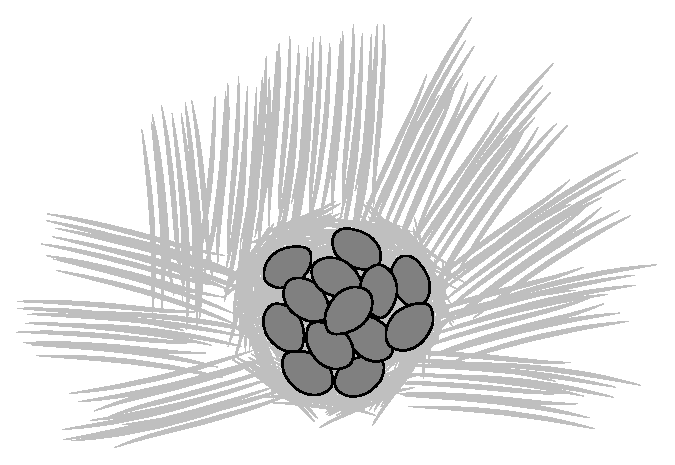
\includegraphics[width=0.40\textwidth]{huevos.eps}
  \end{center}
  \vspace{-20pt}
  %\caption{Figo das índias.}
\end{wrapfigure}
\fi
Algumas vezes, cozinhávamos os ovos, outras vezes os fritávamos; e numa dessas ocasiões, meu pai chegou em casa quando estávamos cozinhando-os,\\\indent
--- e esses ovos?--- perguntou ele, 
e eu, contente e cheio de orgulho, respondi:\\\indent 
--- Zandor achou!\\\indent
Ele meditou um pouco e replicou:\\\indent 
--- Zandor achou... e que coisa deram a ele?\\\indent
A pergunta me pegou de surpresa e falei em voz baixa:\\\indent 
--- Nada pai, só a comida da casa... \\\indent
Meu pai me olhou e falou calmamente: \\\indent
--- Se foi ele quem achou, ele também deve participar.\\\indent
Nesse momento meu pai pegou um ovo cru e deu para o cachorro, Zandor pegou contente o ovo e lambeu até sobrar só a casca. A partir de então, Zandor se acostumou a comê-los sempre que lhe ofereciam. 
Assim, cada vez que ele encontrava ovos, eu os levava para casa, os entregava a minha mãe e ela por sua vez entregava dois a Zandor; porém, nunca lhe dávamos os ovos quando ele os encontrava, somente na casa, ele por sua parte sabia esperar e nunca pegou nenhum, só esperava pacientemente o momento que minha mãe entregasse a ele seus ovos e ia contente a seu cantinho para comê-los.


Para mim, Zandor era maravilhoso, em qualquer lugar aonde eu ia, ele me acompanhava, quando estava triste ele se sentava a meu lado e até chorava comigo fazendo um som agudo, que eu sentia cheio de solidariedade. 
Por outro lado, se ele percebia que eu estava contente, levantava suas orelhinhas e iniciava a pular e correr de um lado a outro. Assim, durante muito tempo, andamos e crescemos juntos... o tempo passou e eu completei oito anos, e logo, nove anos de idade.

Um dia meu pai decidiu abater um boi; lá na serra não se mata um boi sem nenhum motivo, só em ocasiões importantes como festas regionais, casamentos ou eventos semelhantes. No entanto, eu sabia que nessa época não tínhamos nenhuma festividade e pensava que a meu pai simplesmente ocorreu-lhe abater o boi sem nenhum motivo, mas não era assim. 
Eu tinha um irmão mais velho que morava na capital, em Lima; eu não o conhecia, só sabia de sua existência, pois meus pais sempre falavam sobre sua vida lá e se referiam a ele como ``Seve''; nessa época, eu pensava que ele se chamava dessa forma, não obstante, esse não era seu nome e, sim, Severino. Eu não o conhecia porque viajou para Lima quando eu era muito pequeno, seguramente o vi nessa época, mas eu não tinha lembrança alguma. 
Assim, meu pai e minha mãe tinham a intenção de fazer charque para mandar-lhe como encomenda; com essa finalidade, decidiram abater o boi e prepararam cuidadosamente sua carne com muito sal.

\ifdefined\EnableIncludeImages
\begin{wrapfigure}{r}{0.49\textwidth}
  \begin{center}
  \vspace{-20pt}
    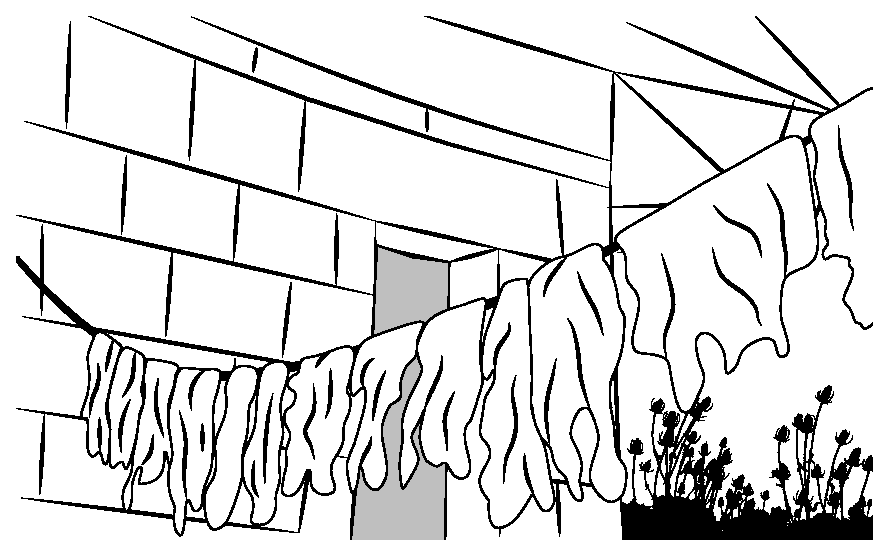
\includegraphics[width=0.47\textwidth]{charque.eps}
  \end{center}
  \vspace{-20pt}
  %\caption{Zandor}
\end{wrapfigure}
\fi
Nosso lar estava composto por uma casa pequena e uma grande, ambas separadas por vários metros entre si; nossa família morava na casa grande e usávamos a pequena para guardar ferramentas, grãos e, em geral, alimentos não perecíveis. 
Perto da casa pequena, nós tínhamos duas figueiras; nesse dia meu pai usou uma delas para amarrar uma corda até a casa pequena, e sobre ela pendurou a carne para secar com o sol; porém, ele decidiu pendurar uma perna de boi no tronco da outra figueira, pois essa peça de carne pesava muito.
Lá o costume é recolher a carne e levá-la para a casa durante a noite, para que os animais de hábitos noturnos não viessem para comê-la, de modo que no dia seguinte, pela manhã, com os primeiros raios do sol, a carne era novamente pendurada; não obstante, nesse dia meu pai recolheu só o charque que estava pendurado na corda e esqueceu a perna que tinha colocado na outra figueira. 
O pior foi que ali, onde meu pai deixou a carne, tranquilamente qualquer cachorro, zorro, ou outro animal carnívoro da serra, poderia pegá-la facilmente, sem a necessidade de pular, uma vez que não estava a muita altura.

Essa noite Zandor não parou de latir; nós, na casa grande, só escutávamos seu barulho com curiosidade, dado que nenhum membro da família lembrou da perna pendurada na figueira. 
Pelo barulho, só reconhecíamos que algumas vezes chegavam outros cachorros, outras vezes não escutávamos nenhum outro animal, só o Zandor latindo com muita raiva e força; meu pai, bravo pelo ruído, só falava:\\\indent
--- Que coisa quer esse cachorro que não nos deixa dormir!\\\indent
Porém, ele não saía da casa grande para indagar sobre a situação. 
Eu tinha muito medo por tudo o que estava acontecendo; pois, na serra, contam histórias dos seres que habitam a noite. 
Alguns diziam que à noite anda o ``cuco''\footnote{Também chamado coca ou coco, este é um ser mítico, uma espécie de fantasma, bruxa ou bicho-papão que anda de noite pelos caminhos.}, e as crianças tinham um terror extremo a esse ser; para piorar a situação, meu pai tinha o costume de contar-nos histórias sobre suas viagens, de como à noite achou o ``cuco'' nos caminhos da serra, ou também que, em algum povoado perto, o ``cuco'' tinha matado algum vizinho, que tinha chupado o sangue de outro ou simplesmente assustado algum caminhante noturno. Devo reconhecer que apesar do terror que me causavam as histórias do meu pai, eu gostava de conhecê-las e passar medo ouvindo-as; ele sempre me contava suas aventuras de quando saía para trabalhar em outras cidades e das coisas que viu, dos problemas que aconteciam no caminho e dos personagens que apareciam quando ele se deslocava a pé.

\ifdefined\EnableIncludeImages
\begin{wrapfigure}{r}{0.49\textwidth}
  \begin{center}
  \vspace{-20pt}
    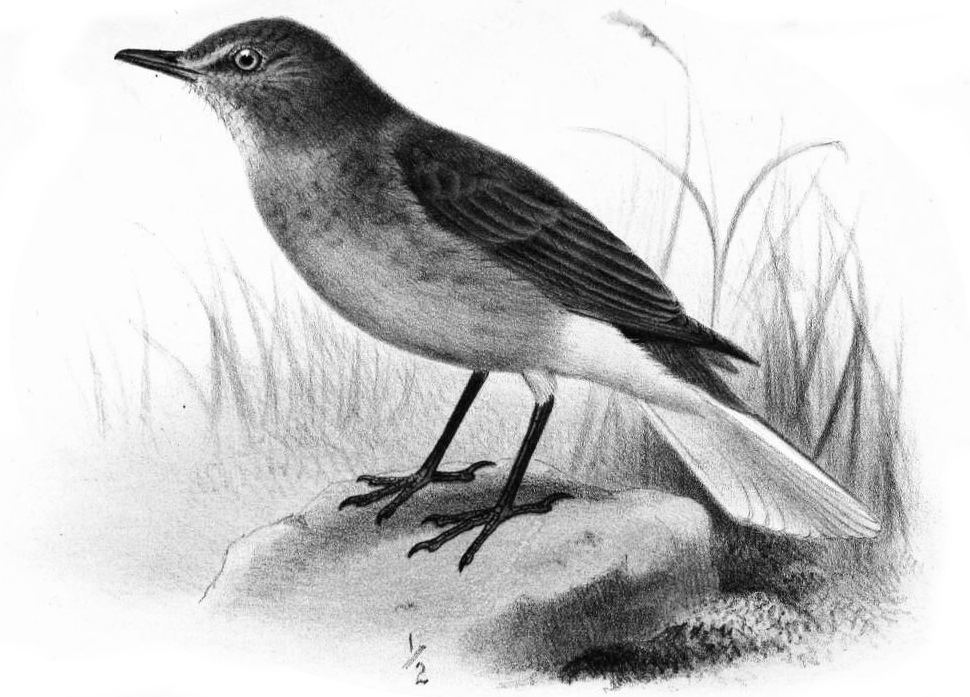
\includegraphics[width=0.47\textwidth]{AgriornisSolitariaSmit.jpg}
  \end{center}
  \vspace{-20pt}
  %\caption{Zandor}
\end{wrapfigure}
\fi
Por exemplo, um dia meu pai me contou que quando estava viajando, caminhando desde nosso povo até ``Cangallo'', um povoado distante, no meio do caminho, a noite chegou, e ele iniciou a procurar entre os trilhos alguma casa que pudesse dar-lhe pousada. Enquanto ele estava nessa tarefa, escutou um pássaro ao qual nós na serra chamamos ``huaychao''\footnote{Também escrito como waychaw, esta é uma palavra quéchua que significa: avisar, anunciar, advertir ou notificar. ``Huaychao'' é uma onomatopeia do som que faz a ave cujo nome científico é Agriornis montanus.}, cujo canto é de mau augúrio.
Meu pai falava que quando o ``Huaychao'' canta, é porque o mal está perto, que ele canta porque viu o mal andando, talvez na forma de algum ``jarjacha''\footnote{Também chamado carcaq ou qarqacha.}. 
Para nós, os ``jarjachas'' são seres da noite, são pessoas que se levantam dos seus túmulos, pois ao terem feito coisas terríveis em vida, estão condenadas a não morrer e vagar de noite entre o sofrimento e a ira. 
Então, meu pai sempre me advertia muito sério que, se na noite escutava ao huaychao, devia ter muito cuidado porque seguramente um ``jarjacha'' estava perto. 
Na sequência dos fatos, quando meu pai escutou ao huaychao, começou a correr pulando pedras e atravessando riachos até que, só e assustado, achou uma casa; rapidamente bateu à porta e de dentro, escutou uma voz de mulher que lhe perguntava:\\\indent
--- Boa noite! Quem está aí?\\\indent
Meu pai, todo assustado, tentou lhe explicar que era só um viajante, que a noite tinha chegado na metade do seu caminho e que somente precisava de um lugar para dormir. A senhora, do interior da casa, respondeu-lhe que, da mesma forma que ele falou, seres que não são pessoas, ``cucos'', andam pela noite enganando os moradores para conseguir entrar em suas casas,\\\indent
--- de repente você é um deles! --- Disse a senhora e negou a meu pai um lugar para dormir.\\\indent
Ele insistiu com a voz tremida pelo medo, porque sabia que tudo isso era verdade, pois ele já tinha escutado ao huaychao e sabia que o mal estava perto. Por fim, após discutir muito, a senhora se comoveu e deixou a meu pai entrar em casa. 
A senhora, toda curiosa pela situação, perguntou a meu pai por que andava à noite, e ele explicou que só estava tentando ir de Occo até Cangalho; porém, teve problemas no caminho e a noite lhe pegou. 
Imediatamente a senhora respondeu em tom maternal:\\\indent 
--- Por que você anda à noite? Só ontem um ``jarjacha'' comeu uma pessoa, agora esse vizinho está morto, hoje mesmo enterramos ele.\\\indent
Por todas essas histórias, sair da casa grande de noite, só porque o cachorro latia, era uma completa temeridade; até meu pai tinha medo de sair, ele só gritava para Zandor de dentro da casa, segurando sua ``guaraca''\footnote{Corda muito versátil que pode ser usada como cinto de calças ou para disciplinar crianças desobedientes.}, golpeando com ela a parede. 
Os demais membros da família, incluindo-me, só escutávamos resignados, tentando dormir apesar do barulho.

Assim, a noite passou, e praticamente nenhum de nós conseguiu dormir. 
Quando os primeiros raios do sol tocaram a nossa janela, todos nós saímos em direção à casa pequena e, para nossa surpresa, vimos a perna de boi pendurada na figueira. 
Para nós foi evidente que, durante a noite, os animais do campo tinham chegado para comer a carne e Zandor tinha defendido-a, brigando, latindo e sem dormir.
\ifdefined\EnableIncludeImages 
\begin{wrapfigure}{r}{0.47\textwidth}
  \begin{center}
  \vspace{-0.5cm}
    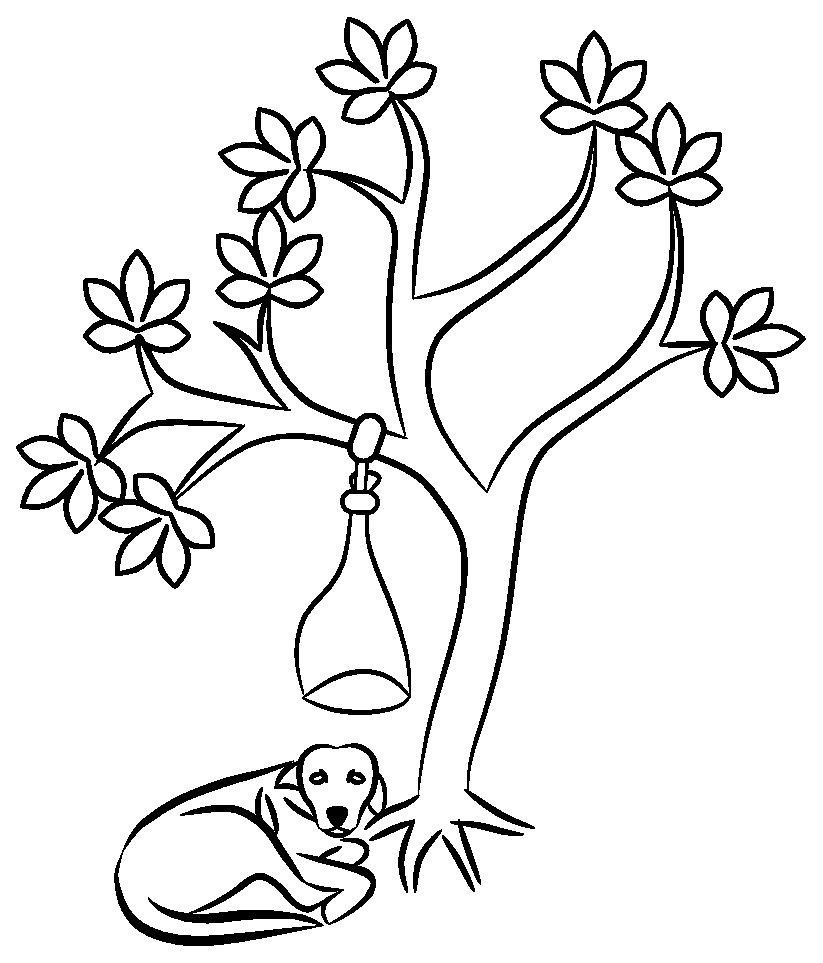
\includegraphics[width=0.45\textwidth]{perro-fiel-1.eps}
  \end{center}
  \vspace{-0.5cm}
  %\caption{Zandor}
\end{wrapfigure}
\fi
Ele estava aconchegado, encolhido em forma de bolinha abaixo da perna de boi e, ao nos ver chegar, só nos dirigiu um olhar cansado enquanto abanava o rabinho. Meu pai se admirou pelo desempenho de Zandor, pois a carne estava intacta.\\\indent
--- Como me esqueci da perna! Por isso chegavam os cachorros! --- exclamou meu pai.\\\indent
Automaticamente entrou na casa, pegou uma faca, cortou um pedaço grande de carne da perna de boi, ainda pendurada na figueira, e a entregou a Zandor como um prêmio; só nesse momento, ele olhou a carne com vontade, pegou seu prêmio e foi para o canto dele para comer.

Assim, Zandor cresceu sendo sempre um cachorro honrado. Se você não dava alguma coisa, ele não pegava; por isso, toda a família o respeitava. Além disso, no campo, os cachorros sempre são bem cuidados; eles comem a mesma comida dos donos de casa e são tratados com carinho, sendo eles considerados como membros da família.

